% Copyright (c) 2021, Julien Seguinot (juseg.github.io), Ian Delaney
% Creative Commons Attribution-ShareAlike 4.0 International License
% (CC BY-SA 4.0, http://creativecommons.org/licenses/by-sa/4.0/)

% Alps erosion paper supplement
% =============================

\documentclass[esurf]{copernicus}

% figures directory
\graphicspath{{../../figures/}}

% document properties
\title{Last glacial cycle glacier erosion potential in the Alps
       \large \newline Supplementary figures}
\Author[1]{Julien}{Seguinot}
\Author[2]{Ian}{Delaney}
\affil[1]{Independent scholar, Anafi, Greece}
\affil[2]{Institute of Earth Surface Dynamics, University of Lausanne, Switzerland}
\runningtitle{Last glacial cycle glacier erosion potential in the Alps}
\runningauthor{J.~Seguinot and I.~Delaney}


% ======================================================================
\begin{document}
% ======================================================================

\nolinenumbers
\onecolumn

    \maketitle

    This document contains copies of the main text Figs. 1--5, and their
    equivalent using the other tested erosion laws.

    \listoffigures

% -- -- -- -- -- -- -- -- -- -- -- -- -- -- -- -- -- -- -- -- -- -- -- -
% Figures
% -- -- -- -- -- -- -- -- -- -- -- -- -- -- -- -- -- -- -- -- -- -- -- -

    \renewcommand\thefigure{S\arabic{figure}}

    \begin{figure*}
      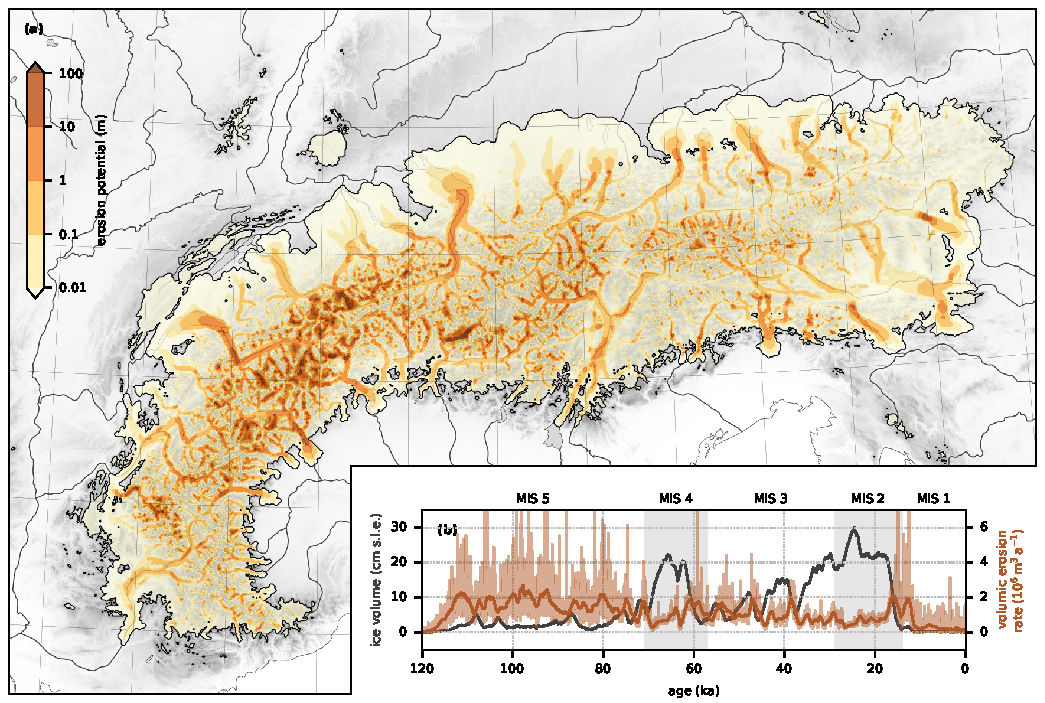
\includegraphics{alpero_cumulative}
      \caption[%
        Cumulative erosion potential and annual erosion volume after
        \citet{Koppes.etal.2015}, same as main text Fig. 1.
        ]{%
        \textbf{(a)} Modelled cumulative (time-integrated) glacial erosion
          potential over the last glacial cycle and geomorphological
          reconstruction of Last Glacial Maximum Alpine glacier extent for
          comparison \citep[solid blue line,][]{Ehlers.etal.2011}.
          The background maps consists of the initial basal topography from
          SRTM \citep{Jarvis.etal.2008} and Natural Earth Data
          \citep{Patterson.Kelso.2017}.
        \textbf{(b)} Modelled total ice volume in centimetres of sea-level
          equivalent (cm~s.l.e., black), annual (domain-integrated) potential
          erosion volume (light brown) and its 1-ka running mean (dark brown).
          Shaded gray areas indicate the timing for MIS~2 and~4
          \citep{Lisiecki.Raymo.2005}. Hatches mark periods with ice volume
          below 3\,cm~s.l.e. where glacier sliding may be affected by
          stress-balance approximations and model horizontal resolution.}
        \label{fig:cumulative}
    \end{figure*}

    \begin{figure*}
      \includegraphics{alpero_cumulative_her2015}
      \caption{%
        Cumulative erosion potential and annual erosion volume after
        \citet{Herman.etal.2015}.}
    \end{figure*}

    \begin{figure*}
      \includegraphics{alpero_cumulative_hum1994}
      \caption{%
        Cumulative erosion potential and annual erosion volume after
        \citet{Humphrey.Raymond.1994}}
    \end{figure*}

    \begin{figure*}
      \includegraphics{alpero_cumulative_coo2020}
      \caption{%
        Cumulative erosion potential and annual erosion volume after
        \citet{Cook.etal.2020}}
    \end{figure*}


% ----------------------------------------------------------------------
% References
% ----------------------------------------------------------------------

%\clearpage
\bibliographystyle{copernicus}
\bibliography{../../../references/references}


% ======================================================================
\end{document}
% ======================================================================
